\documentclass[12pt, a4paper]{report}
\usepackage[]{geometry, scrlayer-scrpage, sectsty, amsmath, amssymb, scrlayer-scrpage, graphicx, listings, xcolor}
\sectionfont{\huge}
\usepackage[onehalfspacing]{setspace}
\geometry{headheight=7.5cm, headsep=1cm}
\geometry{footskip=4.0cm}
\pagestyle{scrheadings}
\ihead{Robotic Games \\\today}
\ohead{Enrico Kaack, Robin Fleige, Laura Nell}
\cfoot{\pagemark}

\definecolor{codegreen}{rgb}{0,0.6,0}
\definecolor{codegray}{rgb}{0.5,0.5,0.5}\documentclass[12pt, a4paper]{report}
\usepackage[]{geometry, scrlayer-scrpage, sectsty, amsmath, amssymb, scrlayer-scrpage, graphicx, listings, xcolor}
\sectionfont{\huge}
\usepackage[onehalfspacing]{setspace}
\geometry{headheight=7.5cm, headsep=1cm}
\geometry{footskip=4.0cm}
\pagestyle{scrheadings}
\ihead{Robotic Games \\\today}
\ohead{Enrico Kaack, Robin Fleige, Laura Nell}
\cfoot{\pagemark}

\definecolor{codegreen}{rgb}{0,0.6,0}
\definecolor{codegray}{rgb}{0.5,0.5,0.5}
\definecolor{codepurple}{rgb}{0.58,0,0.82}
\definecolor{backcolour}{rgb}{0.95,0.95,0.92}

\lstdefinestyle{mystyle}{backgroundcolor=\color{backcolour},   
    commentstyle=\color{codegreen},
    keywordstyle=\color{magenta},
    numberstyle=\tiny\color{codegray},
    stringstyle=\color{codepurple},
    basicstyle=\ttfamily\footnotesize,
    breakatwhitespace=false,         
    breaklines=true,                 
    captionpos=b,                    
    keepspaces=true,                 
    numbers=left,                    
    numbersep=5pt}
    
\lstset{style=mystyle, language=Python}



\begin{document}

\begin{titlepage}

        \centering
        \vspace{1cm}
        {\scshape\Large Robotic Games WS19/20 \par}
        \vspace{1.5cm}
        {\huge\bfseries Zwischenbericht \par}
        \vspace{2cm}
        {\Large\itshape Enrico Kaack, Robin Fleige, Laura Nell \par}

    
        \vfill
    
    % Bottom of the page
        {\large \today\par}
    \end{titlepage}
\newpage    

\pagenumbering{arabic}
\onehalfspacing


\chapter{Implementierung}

\section{Collision avoidance}
Um die Kollisionsvermeidung zu verwirklichen, wird die Momentangeschwindigkeit des Roboters durch einen Subscriber ausgelesen. Zusätzlich sind auf die gleiche Weise die Messwerte der Sonarsensoren in Form von Abständen zum nächsten Hindernis bekannt.
Für die Kollisionsvermeidung wird ein Potentialfeldansatz gewählt, bei welchem die Kraft, welche auf den Roboter durch ein sich näherndes Hindernis ausgeübt wird, die Änderung der Linear- und Winkelgeschwindigkeit bestimmt. Dies ist in der folgenden Funktion \textit{calculate\_force(self, sonar\_angles, sonar\_ranges)} verwirklicht. Dabei handelt es sich bei sonar\_angles um die Winkel zwischen Sensor- und Roboterausrichtung und bei sonar\_ranges um den jeweils zurückgegebenen Abstand.
\begin{lstlisting}
def calculate_force(self, sonar_angles, sonar_ranges):
  sum = np.zeros(2)

  for i, sonar_range in enumerate(sonar_ranges):
      if sonar_range == 0.0:
          rospy.logerr('Catched Zero')
          sonar_range = 1e-12
      vec = np.array([1/sonar_range * np.cos(sonar_angles[i]), 1/sonar_range * np.sin(sonar_angles[i])])
      sum += vec
          
  sum *= (-1)
  sum_dist = np.linalg.norm(sum)
       
  if sum_dist < 10.0:
      return np.zeros(2)

  phi = -np.arctan2(sum[1], sum[0])
  force = np.zeros(2)
  force[0] = np.clip(-sum[0] / 20, 0, 1)
  force[1] = np.clip(phi, -np.pi/2, np.pi/2)

  if -force[1] == self.last_angle:
      force[1] = self.last_angle

  self.last_angle = force[1]
  return force
  
\end{lstlisting}
Um die auf den gesamten Roboter wirkende \''Kraft\'' zu bestimmen, wird die Resultierende aus allen von den Sonarsensoren aufgezeichneten Abstandsvektoren bestimmt. Dazu werden diese in der for-Schleife ab Zeile 4 zunächst in ihre x- und y-Komponenten unterteilt und diese im Array \textit{sum} aufsummiert. Da die \''Kraft\'' entgegen des Roboters wirken soll, wird dieses negiert und anschließend der auf den Roboter wirkende Vektor mithilfe der Funktion \textit{numpy.linalg.norm()} berechnet.\\
Sollte der resultierende Abstand zu einem Hindernis größer als ein bestimmter Wert, hier 10, sein, wird der Fahrtweg des Roboters nicht verändert, es wird ein Nullarray zurückgegeben $($Zeile 14f.$)$.\\
In jedem anderen Fall wird das Array \textit{force[ ]} erstellt und zurückgegeben, wobei \textit{force[0]} die Änderung der Linearbeschleunigung beinhaltet und \textit{force[1]} die Änderung der Winkelbeschleunigung. Die Berechnung der Änderung der Linear- und Winkelbeschleunigung erfolgt mithilfe der Funktion \textit{numpy.clip(a, a\_min, a\_max)}, welche den Wert von a auf das Intervall $[$a\_min, a\_max$]$ beschränkt. Liegt der Wert a unterhalb a\_min, wird a\_min zurückgegeben, liegt a überhalb a\_max, wird a\_max zurückgegeben. \\
Da die Änderung der Lineargeschwindigkeit an den Roboter in der Form 1 - $\Delta$x übermittelt wird, wird der x-Anteil des resultierenden Vektors / 20 hierfür auf das Intervall $[$0,1$]$ begrenzt, da der Roboter nicht rückwärts fahren soll $($negative Linearbeschleunigung$)$ $($Zeile 19$)$. Damit wird die Lineargeschwindigkeit nicht geändert, wenn der Wert x/20 oberhalb von 1 liegt, also der Abstand des Roboters zum Hindernis in x-Richtung noch groß genug ist, und maximal geändert, sollte der Wert negativ sein. Dieser Fall kann allerdings nie eintreten, da dies bedeuten würde, dass der Roboter bereits an/hinter der Wand steht.\\
Die Änderung der Winkelbeschleunigung wird über den negativen arctan2 des resultierenden Vektors, begrenzt auf $[$-$\pi$/2, $\pi$/2$]$, bestimmt $($Zeile 20$)$. Dabei sind die Maximalwerte so gewählt, dass sich der Roboter in einem Schritt nicht zu viel dreht, sondern dies auf mehrere Schritte aufgeteilt wird.\\
Sollte der Roboter genau senkrecht auf eine Ecke zufahren, kann der Fall auftreten, dass die resultierende \''Kraft\'' genau senkrecht auf den Roboter wirkt bzw. dadurch die Änderung der Winkelbeschleunigung zwischen beiden Seiten alterniert, sodass der Roboter sich nicht befreien kann. Dies wird abgefangen, indem die Änderung der Winkelbeschleunigung in diesem Fall auf den positiven Fall festgesetzt wird $($Zeile  22f.$)$.
Die zurückgegebenen Werte werden dem Roboter mithilfe eines Publishers übermittelt.\\


Die Funktionalität des implementierten Programms wird anhand der zur Verfügung gestellten Funktion \textit{create\_visualisation} geprüft und visualisiert. In den folgenden Abbildung sind dessen Ergebnisse gegenübergestellt.\newpage

\begin{centering}
Visualisieriung Welt 1\\
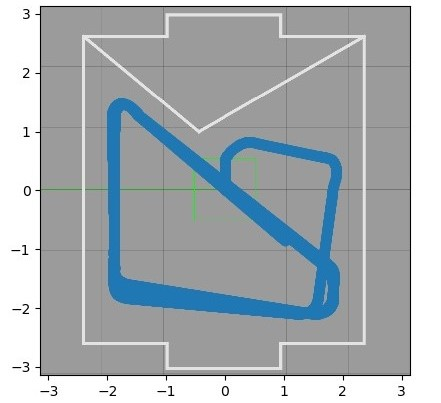
\includegraphics[width=290pt]{roboter_pfad1.jpg}\\
Visualisieriung Welt 2\\
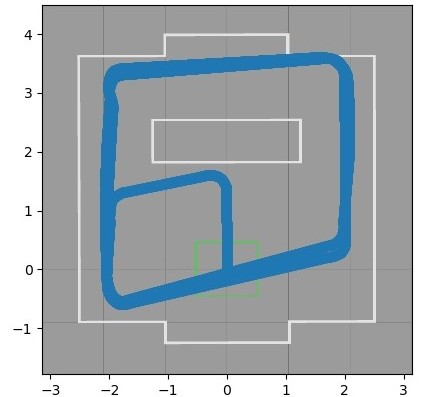
\includegraphics[width=290pt]{roboter_pfad2.jpg}\newpage
~\\
Visualisieriung Welt 3\\
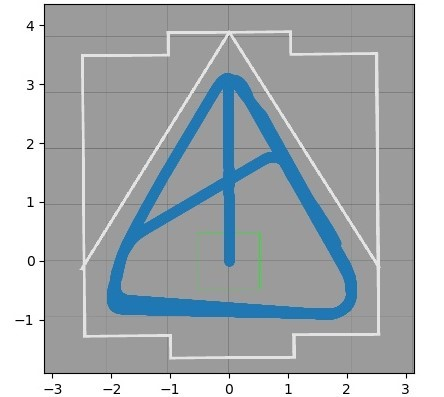
\includegraphics[width=290pt]{roboter_pfad3.jpg}\\
Visualisieriung Welt 4\\
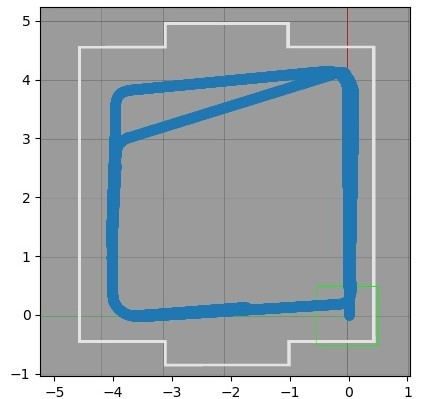
\includegraphics[width=290pt]{roboter_pfad4.jpg}\newpage
~\\
Visualisieriung Welt 5\\
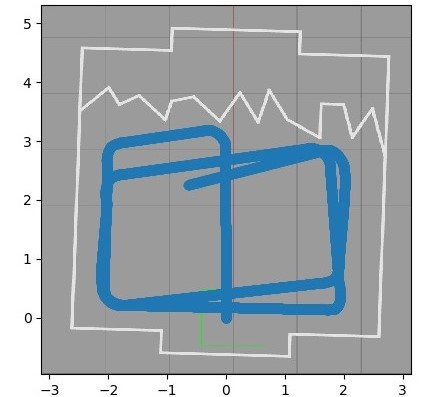
\includegraphics[width=290pt]{roboter_pfad5.jpg}\\
\end{centering}
~\\

Wie in den Abbildungen zu sehen ist, wird die Winkelgeschwindigkeit des Roboters immer um einen bestimmten Wert geändert, sowas der Roboter nach einer Einschwingzeit immer dem gleichen Pfad folgt. Dies ist insbesondere für die Funktionalität der Maus nicht sinnvoll, wird allerdings durch die Verbindung der Kollisionsvermeidung mit den nachfolgend vorgestellten Funktionalitäten verbessert. Ansonsten konnte die Simulation alle getesteten Welten ohne große Probleme meistern, demzufolge wir mit der Implementation der Collision Avoidance weitestgehend zufrieden sind.
\newline

\section{Homing}
Um das Homing umzusetzen, wird die aktuelle Position, die aktuelle Drehung im Raum und die Position des Ziels benötigt. Aus diesen Werten lässt sich berechnen, wie weit und in welche Richtung der Roboter noch fahren muss.\\
Die benötigten Daten werden über einen Subscriber eingelesen. Dieser wird in der folgenden Zeile gestartet. Werden auf dem abonnierten Kanal neue Informationen veröffentlicht, wird ein Callback aufgerufen. 
\begin{lstlisting}
rospy.Subscriber("dead_reckoning", Pose, self.callback)
\end{lstlisting}
Der Callback wird im folgenden Programmabschnitt definiert. Seine einzige Aufgabe ist es, die Positionsdaten sowie die Informationen über die eigene Drehung für den eigentlichen Homing-Algorithmus lesbar zur Verfügung zu stellen. Dies geschieht, indem die Werte in den Instanzvariablen des Homing Objekts gespeichert werden.\\
Da sich der Roboter nur auf der zweidimensionalen Ebene bewegen kann, reichen die x- und y-Koordinate sowie die Drehung um die z-Achse.
\begin{lstlisting}
def callback(self, pos):
  self.orientation[0] = pos.orientation.z
  self.position[0] = pos.position.x
  self.position[1] = pos.position.y
\end{lstlisting}
In \textit{closed\_loop(position,orientation,target)} wird die tatsächliche Berechnung für die Geschwindigkeit sowie die antizipierte Drehung durchgeführt. Die gesamte Funktion wird im folgenden beschrieben und deren tatsächliche Implementierung gezeigt.\\
Zunächst wird ein leeres Objek der Klasse Twistt$()$ erzeugt, in dem anschließend die Werte gespeichert werden (Zeile 2).\\
Anschließend wird für die Dimensionen der x- und y-Achse die relative Position vom Ziel zum Roboter berechnet. Einfacher gesagt berechnen diese zwei Zeilen die Entfernung des Roboters zum Ziel auf der x-Achse und der y-Achse.(Zeile 4f.)\\
Da die Position zunächst in Weltkoordinaten vorliegen, muss diese in Roboterkoordinaten umgerechnet werden, also in Relation zu seiner eigenen Position und Drehung angegeben werden. Dafür wird die relative Position des Ziels zum Roboter um die aktuelle Drehung des Roboters gedreht. Die Koordinaten liegen anschließend so vor, wie sie der Roboter sieht, wenn er sich selbst als Nullpunkt betrachtet.\\
Der Winkel $\alpha$, um welchen sich der Roboter drehen muss, bis er zu seinem Ziel ausgerichtet ist, wird mithilfe des Arcustangens2 der relativen x- und y-Koordinaten im Roboterkoordinatensystem berechnet. Im Code ist dies dargestellt durch \textit{np.arctan2(dir\_x, dir\_y)}.\\
Der Roboter soll sich unter zwei Bedingungen bewegen: 
\begin{itemize}
\item Wenn der noch zu drehende Winkel kleiner ist als $\pi/4$, also 45$^\circ$. 
\item Wenn das Ziel noch mehr als 0.1 Einheiten entfernt ist. 
\end{itemize}
Treten nicht beide Bedingungen ein, wird keine lineare Bewegung ausgeführt $($Zeile 10ff.$)$.\\
Unter der Bedingung, dass die gewünschte Drehung kleiner ist als $\pi/30$, was 6$^\circ$ entspricht, wird eine Rotationsbewegung ausgeführt. Dies wurde als Grenze gewählt, damit der Roboter sich nicht in jedem Zug zwangsweise minimal dreht, um die optimale Drehung zu haben, da dies bei Rauschen dazu führt, dass der Roboter sich deutlich langsamer bewegt. Es ist auch kein Problem, dass sich der Roboter nicht bis 100\% auf das Ziel ausrichtet, da der Winkel zunimmt, wenn der Roboter sich in Richtung Ziel bewegt und somit in jedem Fall eine Korrektur erfolgt, sollte der gefahrene Winkel nicht ausreichen. Um eine fließende Bewegung sicherzustellen, wird der Winkel ein Drittel des gewünschten Winkels geändert.

\begin{lstlisting}
def closed_loop(position,orientation,target):
  output=Twist()

  target_rel_x = target[0] - position[0]
  target_rel_y = target[1] - position[1]

  dir_x = np.cos(orientation[0]-np.pi/2)*target_rel_x + np.sin(orientation[0]-np.pi/2)*target_rel_y
  dir_y = np.cos(orientation[0]-np.pi/2)*target_rel_y - np.sin(orientation[0]-np.pi/2)*target_rel_x

  if np.abs(np.arctan2(dir_x, dir_y)) < np.pi/4 and dir_x*dir_x+dir_y*dir_y > 0.01:
      output.linear.x = 0.5
  else:
      output.linear.x = 0
  if np.abs(np.arctan2(dir_x,dir_y)) > np.pi/30:
      output.angular.z = np.arctan2(dir_x, dir_y)/3

  return output
  
\end{lstlisting}

\newpage
Die implementierte Funktionalität kann, wie bereits bei der Kollisionsvermeidung, mithilfe der Funktion \textit{create\_visualisation} visualisiert und geprüft werden. Im folgenden sind dazu zwei Beispiele mit unterschiedlichen Zielpunkten dargestellt.\newline

\begin{centering}
{\textbf{Zielpunkt $(-3|-2):$}}\\
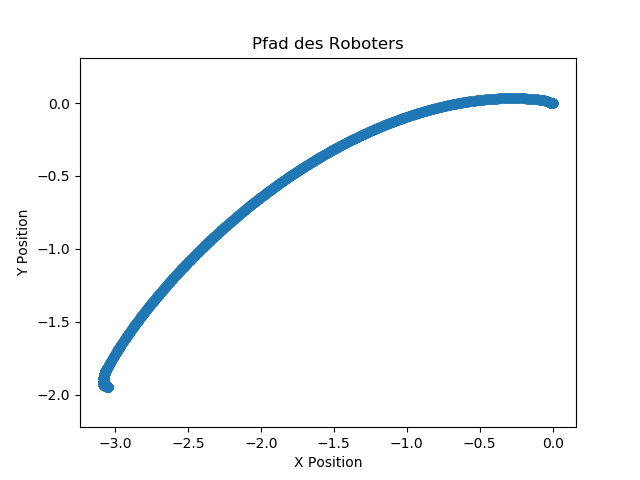
\includegraphics[width=300pt]{homing_example1.png}\\
~\\
{\textbf{Zielpunkt $(2|5):$}}\\
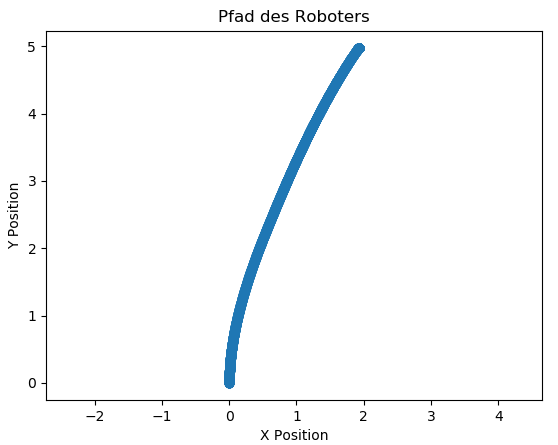
\includegraphics[width=300pt]{homing_example2.png}\\
\end{centering}

Die Ähnlichkeit der beiden Kurven rührt aus der Implenetierung, dass der Roboter sich zunächst bis zu einer bestimmten Ausrichtung in Bezug auf sein Ziel im Stand dreht, bevor er losfährt und die Richtung dabei weiterhin angepasst wird.\newline
In der Sprungantwort der beiden Achsen zu den gegebenen Beispielen sind keine großen Schwankungen zu erkennen, was für die beschriebene Implementierung spricht:\newline

\begin{centering}
{\textbf{Zielpunkt $(-3|-2):$}}\\
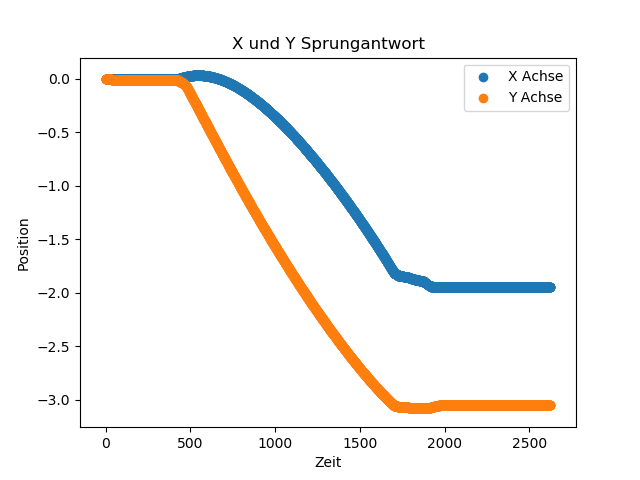
\includegraphics[width=300pt]{Sprungantwort1.png}\\
\newpage
{\textbf{Zielpunkt $(2|5):$}}\\
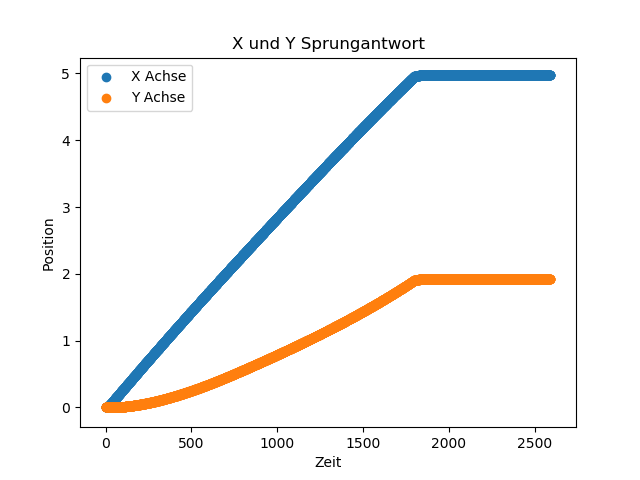
\includegraphics[width=300pt]{Sprungantwort2.png}\\
\end{centering}
~\\

Verbesserung des Homings wäre möglich, wenn der Loop und der Subscriber nicht zwangsläufig gleich getaktet sind, wodurch der Loop möglicherweise mit veralteten Informationen arbeitet, die ein falsches Verhalten hervorrufen. Dies ist jedoch nur schwer zu korrigieren, da bei der Fusion zwei Subscriber Informationen bekommen, man den Loop aber nur auf einen der Subscriber ausrichten kann.\\
Eine weitere Verbesserung wäre, nicht immer um ein Drittel der Zieldrehung zu drehen, da dadurch passieren kann, dass die Drehung in einem kleinen Bereich um 6$^\circ$ hängenbleibt und sich der Roboter dadurch ständig hin- und herdreht, was die Intention der 6$^\circ$ Abfrage zunichte macht. Besser wäre an dieser Stelle eine Funktion, welche für fließende Bewegungen sorgt, jedoch für eine gewünschte Drehung knapp über 6$^\circ$ eine möglichst genaue Drehung auf das Ziel veranlasst. Dadurch würde der Roboter seinen Kurs seltener optimieren müssen, wodurch er schneller vorankommt. Dies soll im folgenden Verlauf so noch realisiert werden.

\section{Free Space}

Das Free Space Verhalten soll dafür sorgen, dass der Roboter in Richtung der größten freien Fläche im Raum fährt. Die zur Verfügung stehenden Informationen beschränken sich dabei wie zuvor auf die vorhandenen acht Ultraschall Sensoren und deren Entfernungsmessung.
\\
Der implementierte Algorithmus prüft, ob die größte Entfernung links oder rechts der Hauptachse gemessen wurde und dreht den Roboter entsprechend nach rechts oder links mit einer konstanten Drehrate. 
\\
Bei diesem Ansatz werden an zwei Stellen Probleme erwartet. Zum einen wird der Sensor mit der maximalen Entfernung zur Bestimmung der Drehrichtung benutzt. Wenn dieser Sensor allerdings einen Gang misst, der vom Roboter weg verläuft, würde sich der Roboter in diese Richtung orientieren. Dieses Verhalten wäre dementsprechend falsch, da der Gang nicht der freien Fläche entspricht. Um dem entgegen zu wirken, könnte man die Sensorwerte von jeweils der rechten und linken Seite mitteln und darauf basierend die Richtungsentscheidung treffen. Im späteren Schritt der Fusion wird der Free Space Teil allerdings nur eine untergeordnete Rolle spielen, sodass dieses Problem nicht in dieser Form auftritt.\\
Eine zweite Schwäche liegt darin, dass eine konstante Drehrate in die jeweilige Richtung gesetzt wird. Eine Auswirkung hiervon wäre, dass bei zu hoher Geschiwndigkeit der Roboter gegen ein Hindernis fahren könnte, da die konstante Drehrate nicht auf die Lineargeschwindigkeit angepasst ist und der Kurvenradius demnach größer wird. Eine Lineargeschwindigkeit abhängig von der Entfernung des Sensors mit der niedrigsten Entfernung würde dies beheben. Sollte in der Fusion dies zu einem Problem führen, wird diese Idee entsprechend aufgegriffen. Da allerdings die Kollisionsvermeidung eine höhere Gewichtung in der Nähe einer Wand erhalten wird, sollte dies nicht zu einem Problem führen.


\section{Verhaltensfusion}
Die Verhaltensfusion beschreibt die Kombination der einzelnen Steuerungsinformationen auf der Kollisionsvermeidung, der Free Space Orientierung und der Zielsuche. Hierdurch soll der Roboter sich in Richtung des Ziels (Zielsuche) durch den Raum bewegen können, ohne mit anderen Objekten zu kollidieren (Kollisionsvermeidung) oder in Sackgassen festzustecken (Free Space).
\\
Ein Ansatz hierfür ist die Verwendung von analogen Schaltern (Gates). Folgende Schalter stehen zur Verfügung:
\begin{description}
    \item[AND-Gate] Das analoge AND Gate funktioniert ähnlich dem logischen AND Gate. Die Ausgabe wächst am schnellsten, wenn beide Eingaben gleichmäßig wachsen. Wenn eine Eingabe 0 ist, gibt es keine Ausgabe.
    \item[OR-Gate] Die Ausgabe des analogen OR-Gates wird von der Größe beider Eingaben bestimmt. Wenn eine Eingabe 0 ist, so wird die andere Eingabe ausgegeben.
    \item[XOR-Gate] Wenn beide Eingaben gleich groß sind, wird die Ausgabe 0 sein. ISt eine Eingabe 0, so ist die Ausgabe gleich der anderen Eingabe.
    \item[Invoke-Gate] Das Invoke-Gate zeigt ein asymetrisches Verhalten. Wenn die Eingabe x steigt, so steigt der Anteil der Eingabe y am Ausgang. Ist die Eingabe x nicht vorhanden, so ist die Ausgabe 0. Ist Eingabe y hingegen 0, wird Eingabe x als Ausgabe genommen.
    \item[Prevail-Gate]  Wenn Eingabe x 0 ist, wird Eingabe y als Ausgabe genommen. Wenn allerdings x ungleich 0 ist, so dominiert die Eingabe x die Ausgabe.
\end{description}   

Es gibt zwei verschiedene Datensätze, die in die analogen Gates gegeben werden können. Zum einen kann für jedes Einzelverhalten die berechnete Kraft auf den Roboter fusioniert werden und die Ausgabe in Lineargeschwindigkeit und Winkelgeschwindigkeit umgerechnet werden. Zum anderen kann die in jedem Einzelverhalten berechnete Lineargeschwindigkeit und Winkelgeschwindigkeit durch zwei Netzwerke geleitet werden. Die vorliegende Implementierung setzt auf letzteren Ansatz. Die damit einhergehende Probleme werden im Folgenden diskutiert.
\subsection{erste Iteration}
Der erste Ansatz (vgl. \ref{listing:erstesNetzwerk}) besteht aus einer AND Kombination der Zielsuche und des Free Space mit einer darauffolgenden INVOKE Kombination mit der Kollisionsvermeidung. Letzeres Gate soll dafür sorgen, dass die Kollisionsvermeidung keinen Beitrag liefert, solange diese 0 ist. Wenn allerdings ein stärker werdendes Signal der Kollisionsvermeidung geschickt wird, so soll dieses stärker berücksichtigt werden.
\begin{figure}
    \begin{lstlisting}

    Homing --------|
                  AND---------|  
    Free Space ----|          |x
                            INVOKE ---------> OUTPUT    
    Collision voidance -------|y
    \end{lstlisting}
    \caption{Netzwerk Verhaltensfusion in erster Iteration (für Lineargeschwindigkeit und Winkelgeschwindigkeit)}
    \label{listing:erstesNetzwerk}
\end{figure}
Praktisches Problem hierbei ist allerdings, dass eine Kollision nicht zuverlässig vermieden werden kann. Grund hierfür liegt in der Lineargeschwindigkeit, die in der Ausgabe nicht 0 ist, auch wenn die Kollisionsvermeidung die Lineargeschwindigkeit auf 0 setzt (siehe Eigenschaften Invoke-Gate).
\subsection{zweite Iteration}
\begin{figure}
    \begin{lstlisting}

    Homing --------|
                  AND---------|  
    Free Space ----|          |y
                            INVOKE ----> LINEARGESCHWINDIGKEIT   
    Collision voidance -------|x
------------------------------------------------------------------
    Homing --------|
                  AND---------|  
    Free Space ----|          |y
                            PREVAIL ----> WINKELGESCHWINDIGKEIT   
    Collision voidance -------|x
    \end{lstlisting}
    \caption{Netzwerk Verhaltensfusion in zweiter Iteration}
    \label{listing:zweitesNetzwerk}
\end{figure}
In der zweiten Iteration (siehe \ref{listing:zweitesNetzwerk}) werden die Lineargeschwindigkeit und die Winkelgeschwindigkeit über zwei verschiedene Netze geregelt. Für die Regelung der Lineargeschwindigkeit wird nun die Kollisionsvermeidung als x Eingabe in das Invoke Gate geführt. Die Kollisionsvermeidung gibt Lineargeschwindigkeit 1 solange kein Grund zum Eingreifen besteht und Lineargeschwindigkeit 0 wenn die Kollisionsvermeidung eingreifen muss. Durch den Anschluss als Eingabe x wird die resultierende Lineargeschwindigkeit unterdrückt, wenn die Kollisionsvermeidung keine Lineargeschwindigkeit zulässt. Ansonsten wird die Lineargeschwindigkeit durch die Zielsuche und Free Space geregelt.
\\
Für die Winkelgeschwindigkeit gilt das Gegenteilige Prinzip. Wenn die Kollisionsvermeidung einen Winkelgeschwindigkeit vorgibt, dominiert dies die Ausgabe der Winkelgeschwindigkeit. Ansonsten wird die Ausgabe der Zielsuche und des Free Space genommen.
\\
Mehrere Dinge müssen bei der Kombination beachtet werden, damit die Ausgabe korrekt ist. Die Eingabedimension muss vergleichbar sein. Das bedeutet, dass alle Eingaben vergleichbar mit ihrer Wichtigkeit skalieren. Möglich wird dies durch entsprechende Anpassung in den Einzelverhalten, sodass diese vergleichbarere Werte produzieren. Darüberhinaus müssen widersprüchliche Informationen sinnvoll verarbeitet werden (Zielsuche: Drehung nach rechts, Free Space: Drehung nach links). Dies ist in der aktuellen Implementierung noch unzureichend beachtet (siehe \ref{chap:ausblick})

\subsubsection{Ergebnisse}
\begin{figure}[]
    \centering
    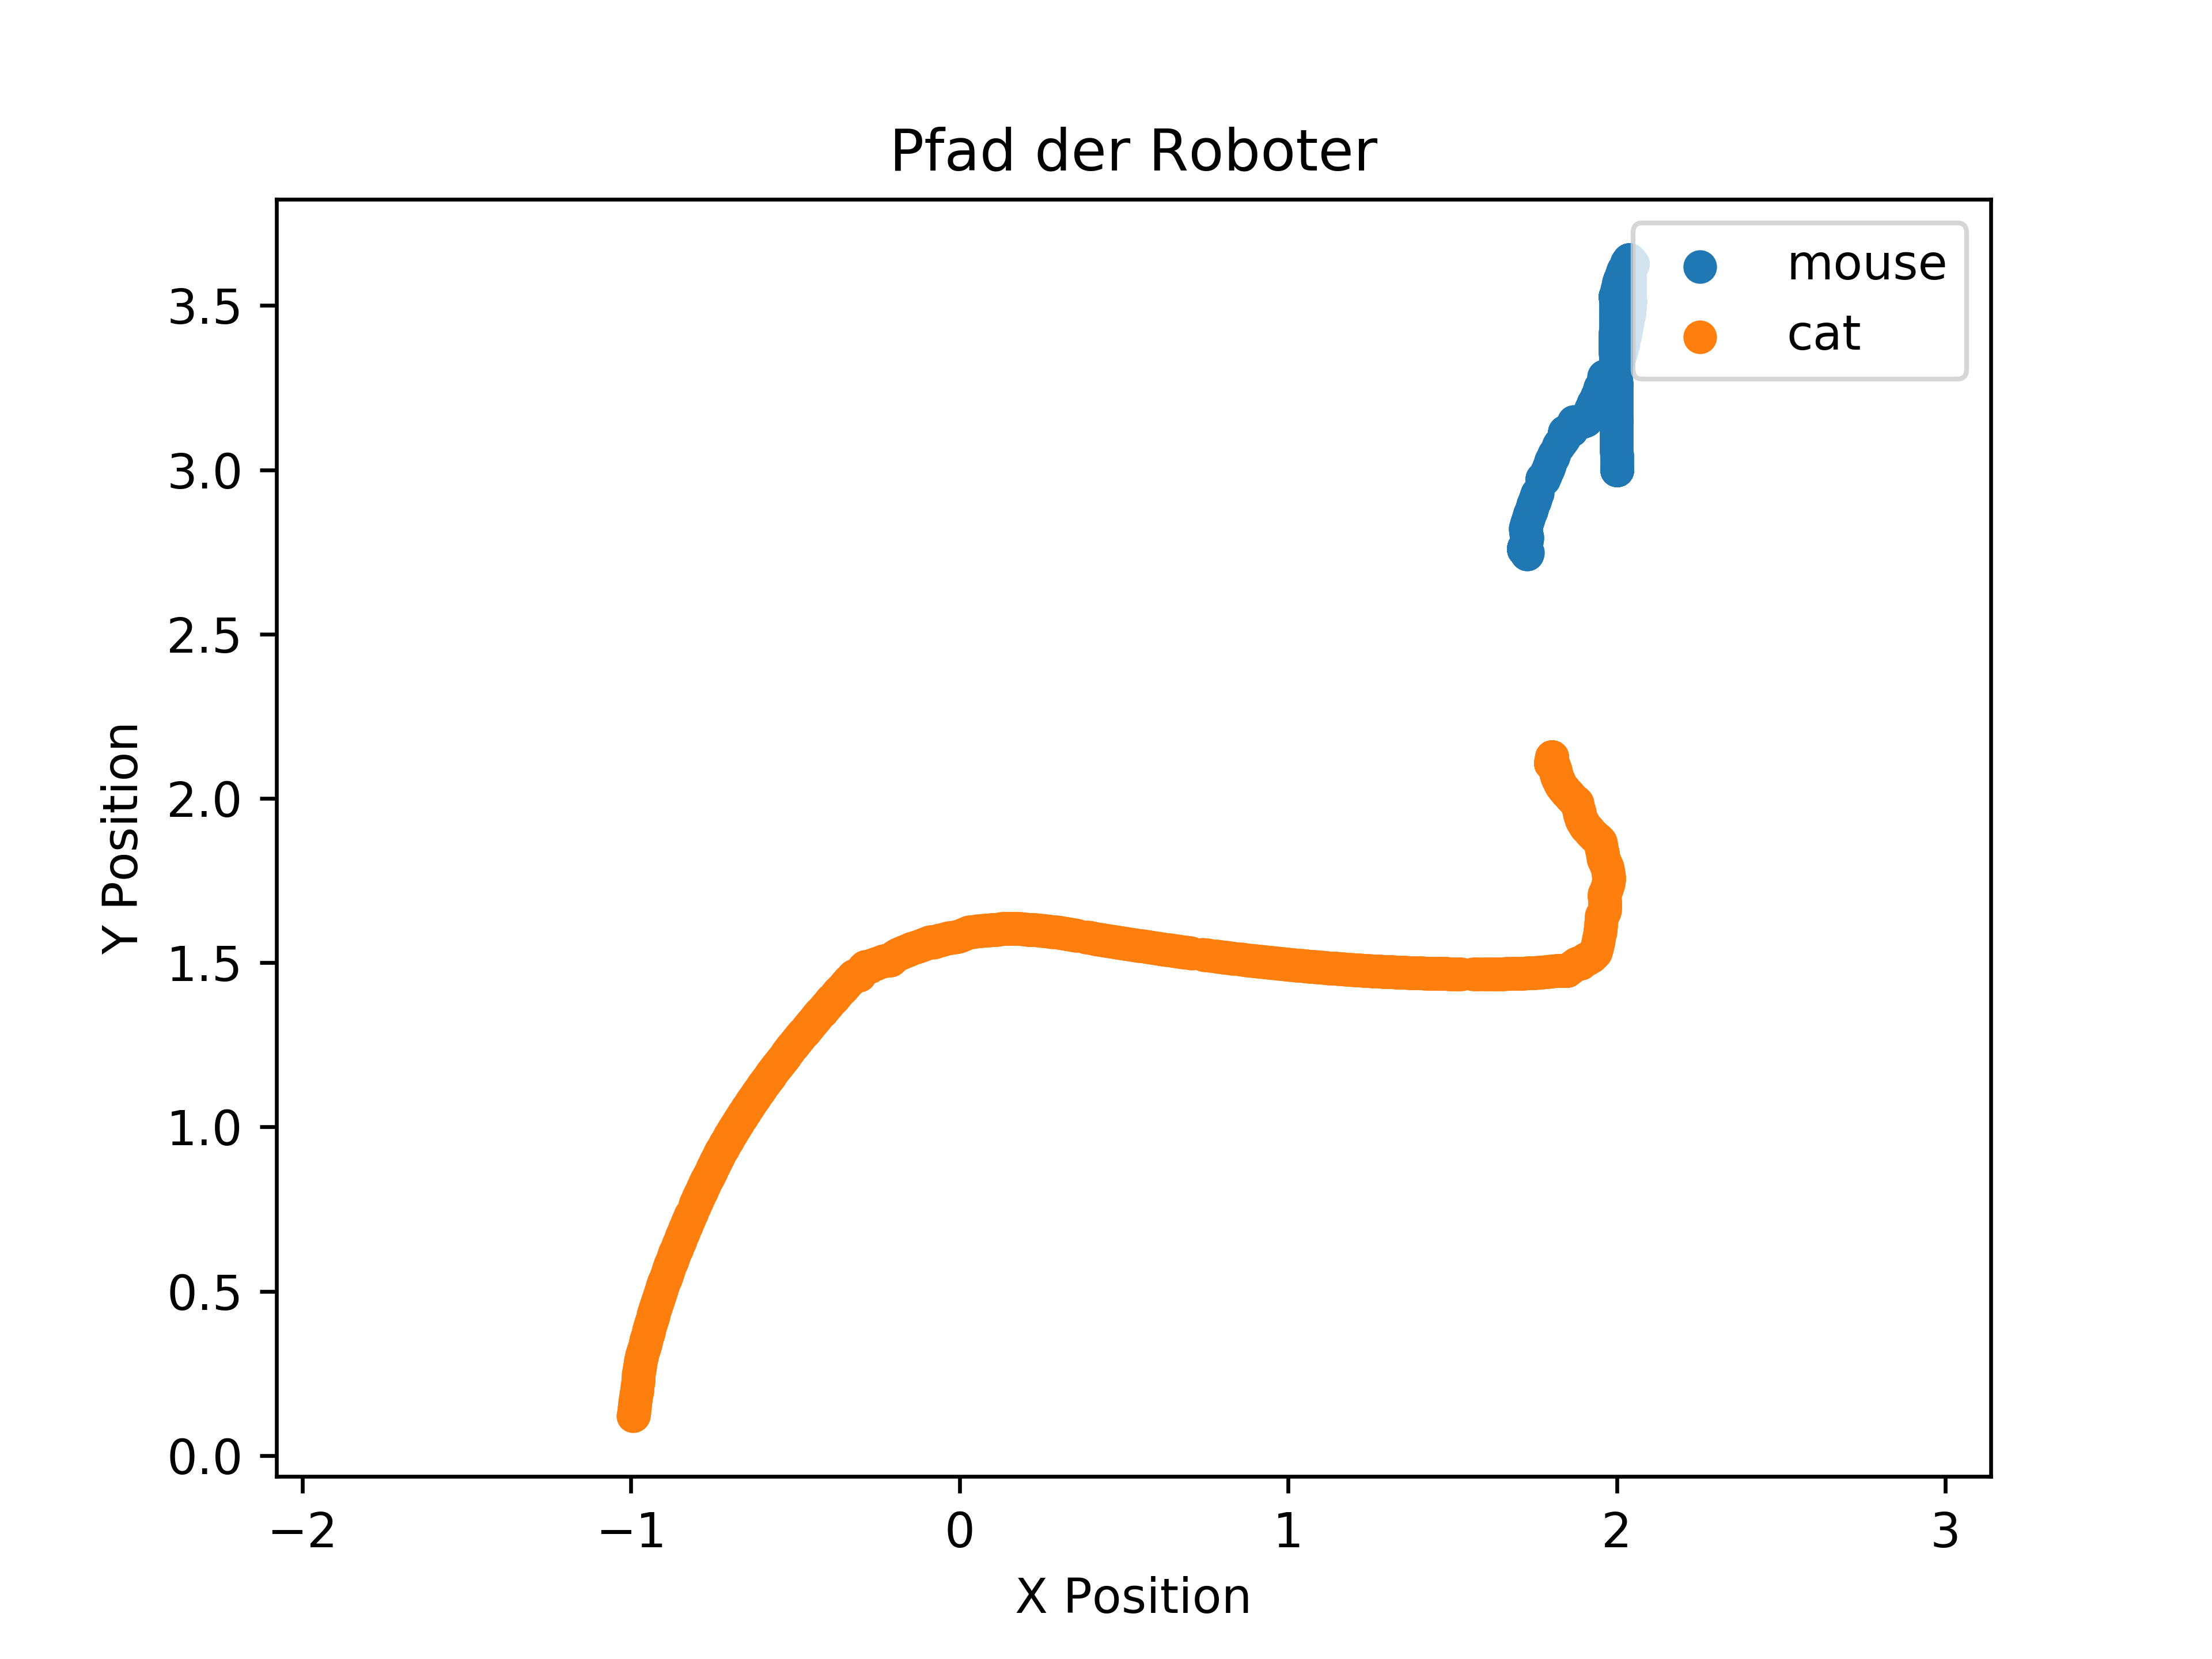
\includegraphics[width=\textwidth]{report_pfad.png}
    \caption{Pfad der Roboter bei Verhaltensfusion}
    \label{fig:pfadFusion}
\end{figure}
\begin{figure}[]
    \centering
    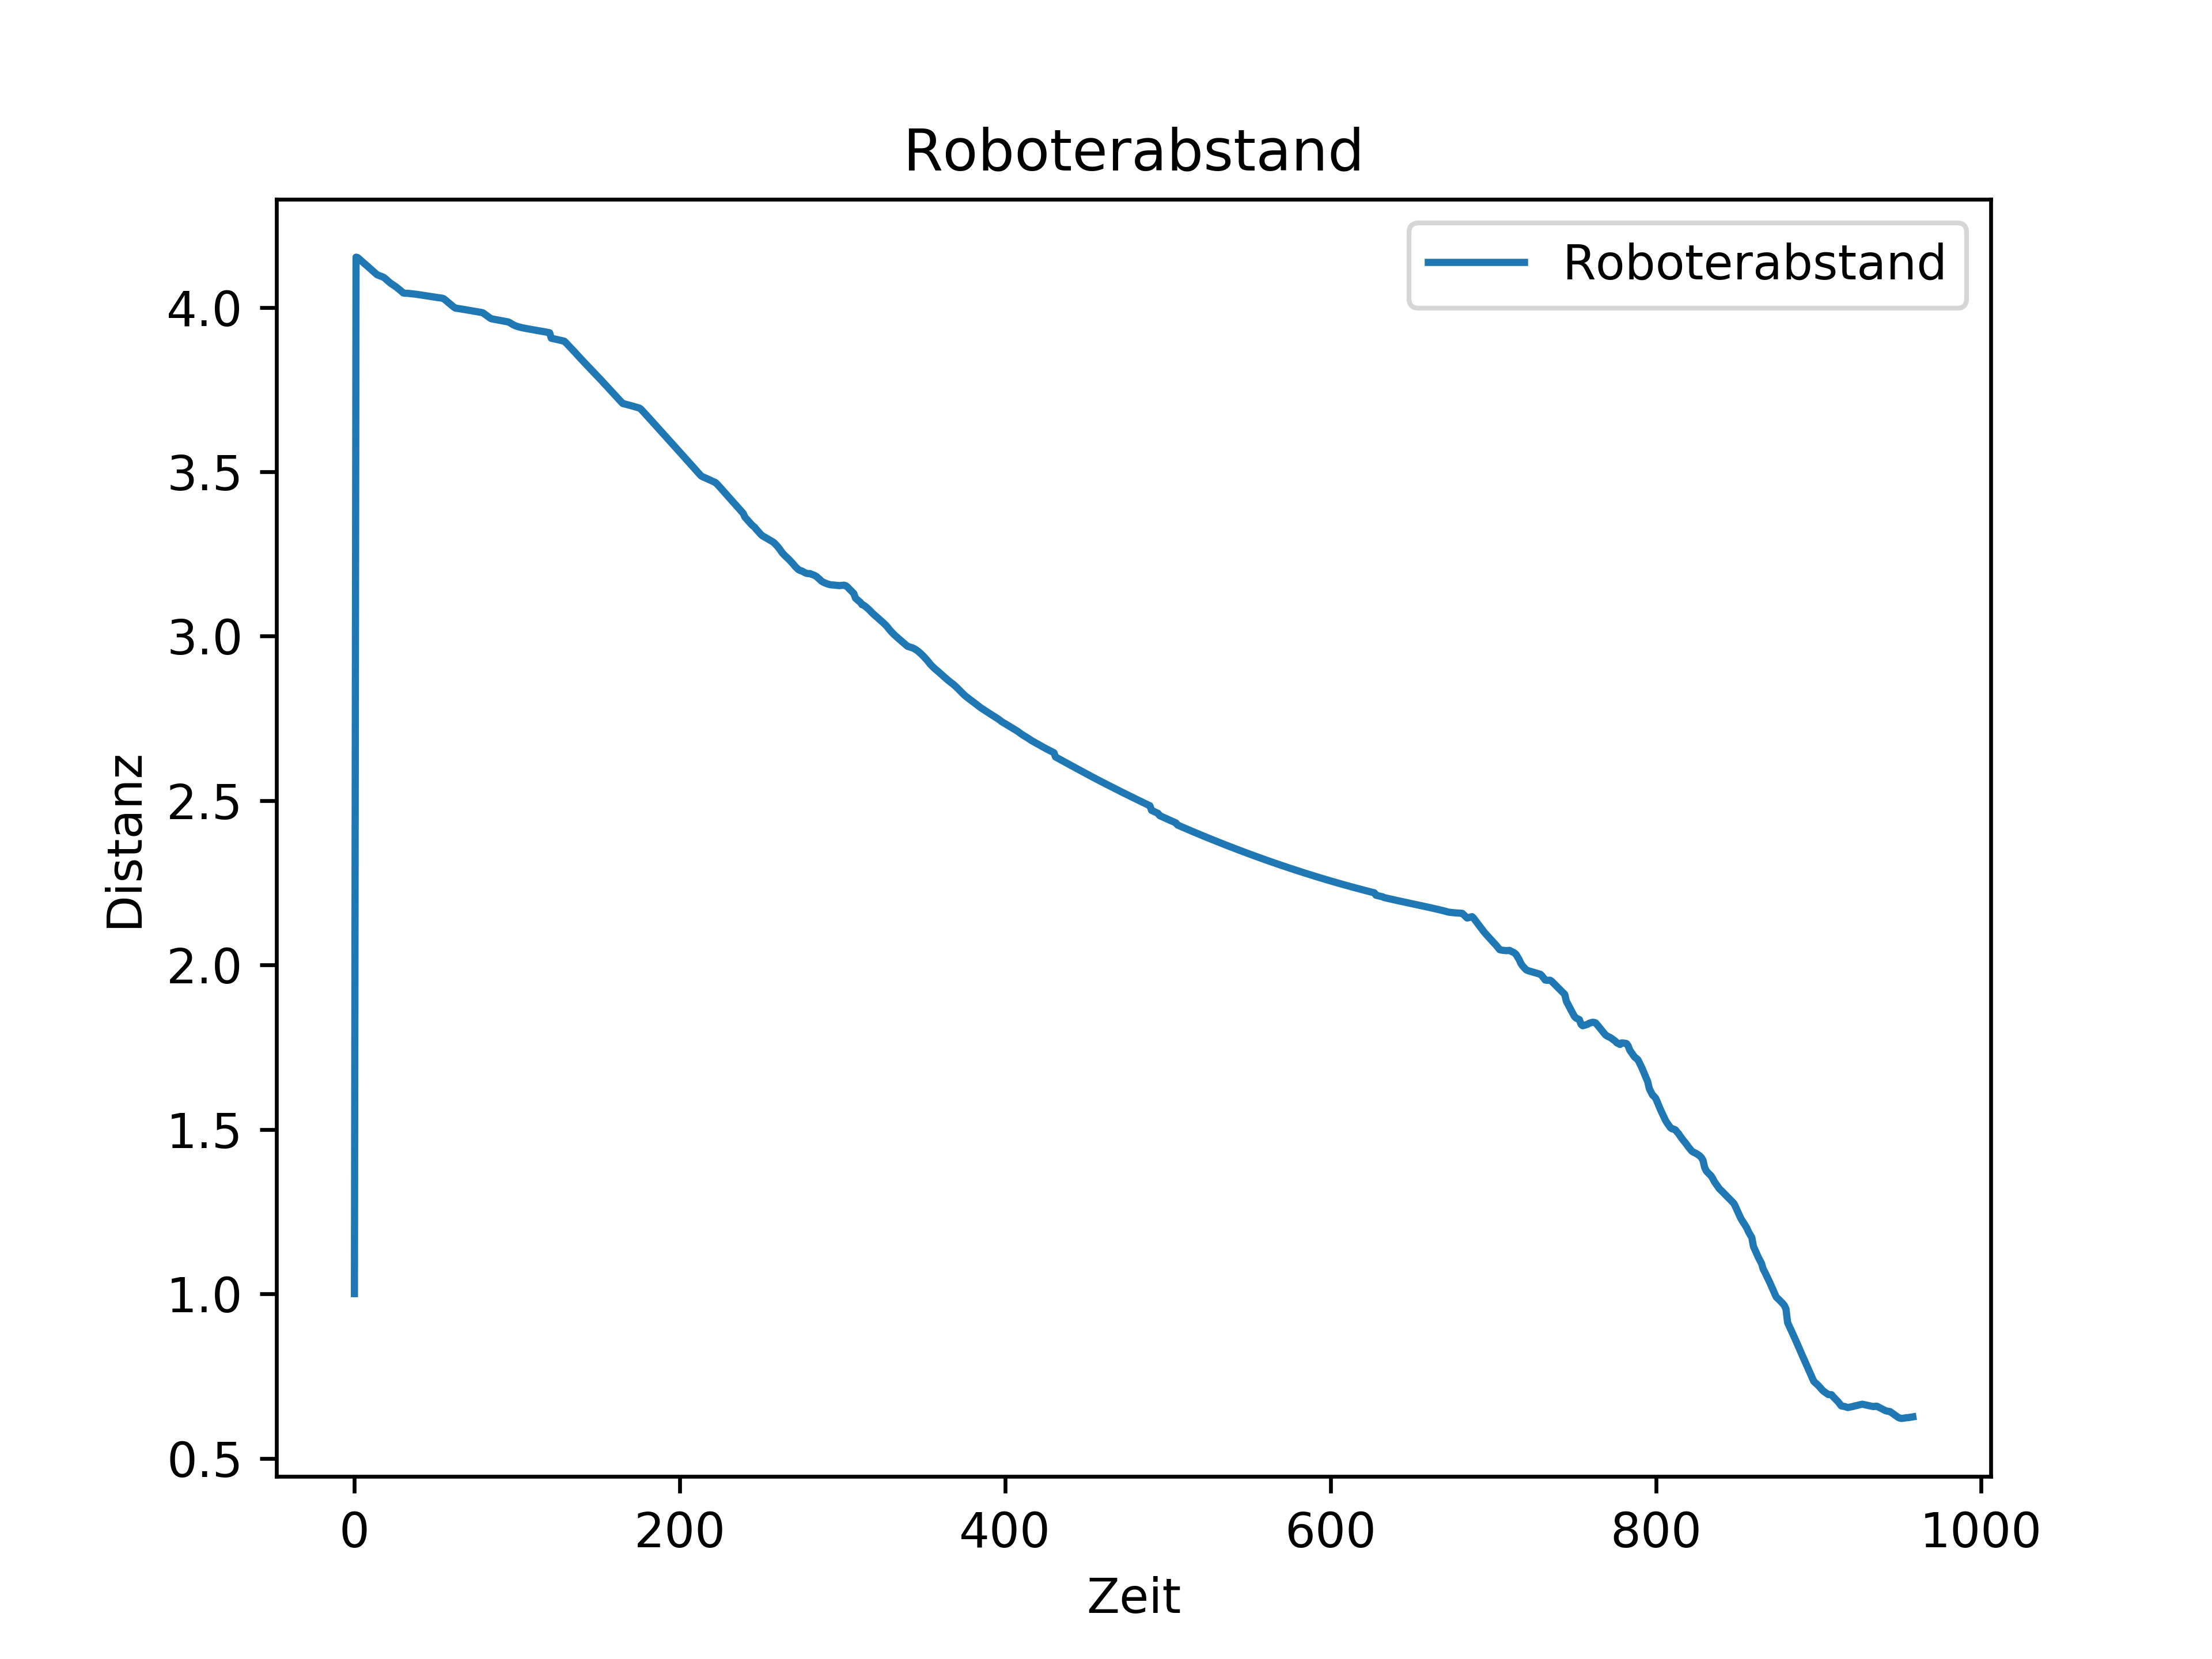
\includegraphics[width=\textwidth]{report_distance.png}
    \caption{Entfernung zwischen den Robotern}
    \label{fig:distanceFusion}
\end{figure}
Der Pfad der Katze in \ref{fig:pfadFusion} verläuft optimal, um die Maus zu erreichen. Bei 0|2 bis ungefähr 1.5|2 begindet sich ein Hinderniss, das umfahren wird, um dann wieder zur Maus aufzuschließen. Dies zeigt sich auch in der linear kleiner werdenden Entfernung zwischen den beiden Robotern. Die Distanz wird nicht auf 0 runter gehen, da in der aktuellen Implementierung die Maus auch als Hindernis erkannt wird und demnach die Kollisionsvermeidung Vorrang erhält, wenn sich die Katze zu sehr der Maus annähert.


\subsection*{Ausblick} \label{chap:ausblick}
Ein sinnvoller Ansatz, der evaluiert werden kann, besteht in der Benutzung von Zusammengesetzten (Compound) Netzwerken. Dabei befindet sich der Roboter in verschiedenen Modi und hat je nach Modi unterschiedliche Verhaltensfusionen. Ein Modus wäre beispielsweise ein direkter Sichtkontakt zur Maus, sodass die Kollisionsvermeidung ausgeschaltet werden kann und die Katze näher an die Maus heranfahren kann. Im Modus Sichtkontakt unterbrochen würde wiederum die Kollisionsvermeidung aktiv werden und gleichzeitig werden Free Space und Zielsuche anders gewichtet.
\\
Ein weiterer Schritt könnte natürlich sein, einen SLAM Algorithmus zu entwickeln, um während der Verfolgung die Umgebung zu scannen und dann nach genug Informationen über den Raum keine Zielsuche mehr durchzuführen sondern eine Wegplanung über bpsw. einen gitterbasierten Dijkstra Ansatz erfolgt.

\end{document}
\definecolor{codepurple}{rgb}{0.58,0,0.82}
\definecolor{backcolour}{rgb}{0.95,0.95,0.92}

\lstdefinestyle{mystyle}{backgroundcolor=\color{backcolour},   
    commentstyle=\color{codegreen},
    keywordstyle=\color{magenta},
    numberstyle=\tiny\color{codegray},
    stringstyle=\color{codepurple},
    basicstyle=\ttfamily\footnotesize,
    breakatwhitespace=false,         
    breaklines=true,                 
    captionpos=b,                    
    keepspaces=true,                 
    numbers=left,                    
    numbersep=5pt}
    
\lstset{style=mystyle, language=Python}



\begin{document}

\begin{titlepage}

        \centering
        \vspace{1cm}
        {\scshape\Large Robotic Games WS19/20 \par}
        \vspace{1.5cm}
        {\huge\bfseries Zwischenbericht \par}
        \vspace{2cm}
        {\Large\itshape Enrico Kaack, Robin Fleige, Laura Nell \par}

    
        \vfill
    
    % Bottom of the page
        {\large \today\par}
    \end{titlepage}
\newpage    

\pagenumbering{arabic}
\onehalfspacing


\chapter{Implementierung}

\section{Collision avoidance}
Um die Kollisionsvermeidung zu verwirklichen, wird die Momentangeschwindigkeit des Roboters durch einen Subscriber ausgelesen. Zusätzlich sind auf die gleiche Weise die Messwerte der Sonarsensoren in Form von Abständen zum nächsten Hindernis bekannt.
Für die Kollisionsvermeidung wird ein Potentialfeldansatz gewählt, bei welchem die Kraft, welche auf den Roboter durch ein sich näherndes Hindernis ausgeübt wird, die Änderung der Linear- und Winkelgeschwindigkeit bestimmt. Dies ist in der folgenden Funktion \textit{calculate\_force(self, sonar\_angles, sonar\_ranges)} verwirklicht. Dabei handelt es sich bei sonar\_angles um die Winkelzwischen Sensor- und Roboterausrichtung und bei sonar\_ranges um den jeweils zurückgegebenen Abstand.
\begin{lstlisting}
def calculate_force(self, sonar_angles, sonar_ranges):
  sum = np.zeros(2)

  for i, sonar_range in enumerate(sonar_ranges):
      if sonar_range == 0.0:
          rospy.logerr('Catched Zero')
          sonar_range = 1e-12
      vec = np.array([1/sonar_range * np.cos(sonar_angles[i]), 1/sonar_range * np.sin(sonar_angles[i])])
      sum += vec
          
  sum *= (-1)
  sum_dist = np.linalg.norm(sum)
       
  if sum_dist < 10.0:
      return np.zeros(2)

  phi = -np.arctan2(sum[1], sum[0])
  force = np.zeros(2)
  force[0] = np.clip(-sum[0] / 20, 0, 1)
  force[1] = np.clip(phi, -np.pi/2, np.pi/2)

  if -force[1] == self.last_angle:
      force[1] = self.last_angle

  self.last_angle = force[1]
  return force
  
\end{lstlisting}
Um die auf den gesamten Roboter wirkende \''Kraft\'' zu bestimmen, wird die Resultierende aus allen von den Sonarsensoren aufgezeichneten Abstandsvektoren bestimmt. Dazu werden diese in der for-Schleife ab Zeile 4 zunächst in ihre x- und y-Komponenten unterteilt und diese im Array \textit{sum} aufsummiert. Da die \''Kraft\'' entgegen des Roboters wirken soll, wird dieses negiert und anschließend der auf den Roboter wirkende Vektor mithilfe der Funktion \textit{numpy.linalg.norm()} berechnet.\\
Sollte der resultierende Abstand zu einem Hindernis größer als ein bestimmter Wert, hier 10, sein, wird der Fahrtweg des Roboters nicht verändert, es wird ein Nullarray zurückgegeben $($Zeile 14f.$)$.\\
In jedem anderen Fall wird das Array \textit{force[ ]} erstellt und zurückgegeben, wobei \textit{force[0]} die Änderung der Linearbeschleunigung beinhaltet und \textit{force[1]} die Änderung der Winkelbeschleunigung. Die Berechnung der Änderung der Linear- und Winkelbeschleunigung erfolgt mithilfe der Funktion \textit{numpy.clip(a, a\_min, a\_max)}, welche den Wert von a auf das Intervall $[$a\_min, a\_max$]$ beschränkt. Liegt der Wert a unterhalb a\_min, wird a\_min zurückgegeben, liegt a überhalb a\_max, wird a\_max zurückgegeben. \\
Da die Änderung der Lineargeschwindigkeit an den Roboter in der Form 1 - $\Delta$x übermittelt wird, wird der x-Anteil des resultierenden Vektors / 20 hierfür auf das Intervall $[$0,1$]$ begrenzt, da der Roboter nicht rückwärts fahren soll $($negative Linearbeschleunigung$)$ $($Zeile 19$)$. Damit wird die Lineargeschwindigkeit nicht geändert, wenn der Wert x/20 oberhalb von 1 liegt, also der Abstand des Roboters zum Hindernis in x-Richtung noch groß genug ist, und maximal geändert, sollte der Wert negativ sein. Dieser Fall kann allerdings nie eintreten, da dies bedeuten würde, dass der Roboter bereits an/hinter der Wand steht.\\
Die Änderung der Winkelbeschleunigung wird über den negativen arctan2 des resultierenden Vektors, begrenzt auf $[$-$\pi$/2, $\pi$/2$]$, bestimmt $($Zeile 20$)$. Dabei sind die Maximalwerte so gewählt, dass sich der Roboter in einem Schritt nicht zu viel dreht, sondern dies auf mehrere Schritte aufgeteilt wird.\\
Sollte der Roboter genau senkrecht auf eine Ecke zufahren, kann der Fall auftreten, dass die resultierende \''Kraft\'' genau senkrecht auf den Roboter wirkt bzw. dadurch die Änderung der Winkelbeschleunigung zwischen beiden Seiten alterniert, sodass der Roboter sich nicht befreien kann. Dies wird abgefangen, indem die Änderung der Winkelbeschleunigung in diesem Fall auf den positiven Fall festgesetzt wird $($Zeile  22f.$)$.
Die zurückgegebenen Werte werden dem Roboter mithilfe eines Publishers übermittelt.\\


Die Funktionalität des implementierten Programms wird anhand der zur Verfügung gestellten Funktion \textit{create\_visualisation} geprüft und visualisiert. In den folgenden Abbildung sind dessen Ergebnisse gegenübergestellt.\newpage

\begin{centering}
Visualisieriung Welt 1\\
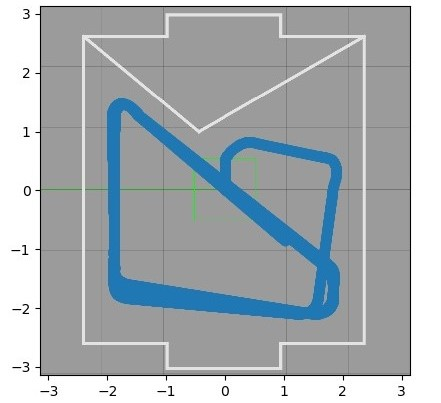
\includegraphics[width=290pt]{roboter_pfad1.jpg}\\
Visualisieriung Welt 2\\
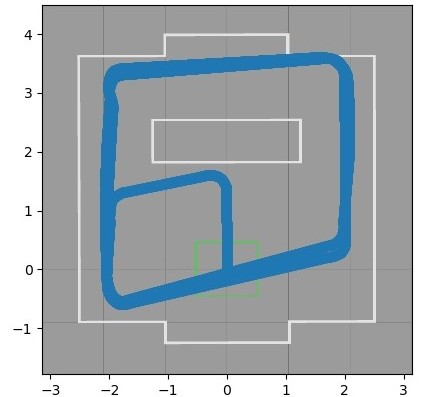
\includegraphics[width=290pt]{roboter_pfad2.jpg}\newpage
~\\
Visualisieriung Welt 3\\
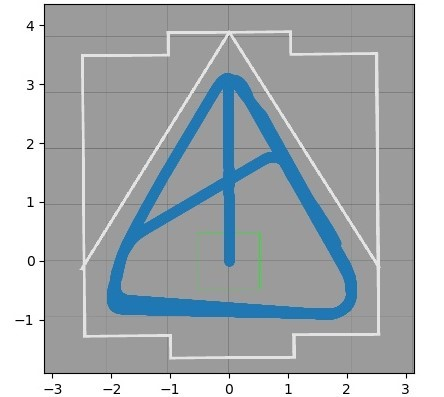
\includegraphics[width=290pt]{roboter_pfad3.jpg}\\
Visualisieriung Welt 4\\
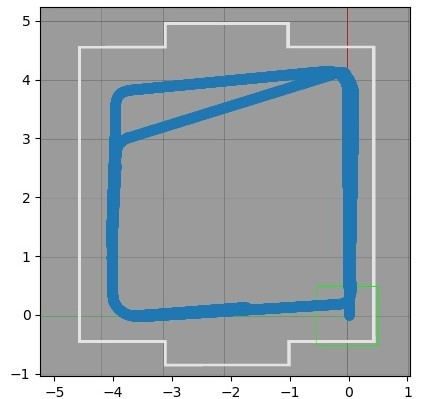
\includegraphics[width=290pt]{roboter_pfad4.jpg}\newpage
~\\
Visualisieriung Welt 5\\
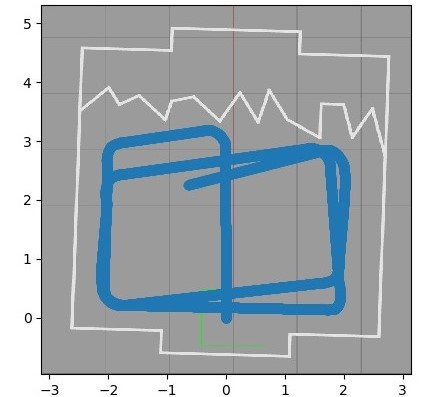
\includegraphics[width=290pt]{roboter_pfad5.jpg}\\
\end{centering}
~\\

Wie in den Abbildungen zu sehen ist, wird die Winkelgeschwindigkeit des Roboters immer um einen bestimmten Wert geändert, sowas der Roboter nach einer Einschwingzeit immer dem gleichen Pfad folgt. Dies ist insbesondere für die Funktionalität der Maus nicht sinnvoll, wird allerdings durch die Verbindung der Kollisionsvermeidung mit den nachfolgend vorgestellten Funktionalitäten verbessert. Ansonsten konnte die Simulation alle getesteten Welten ohne große Probleme meistern, demzufolge wir mit der Implementation der Collision Avoidance weitestgehend zufrieden sind.
\newline

\section{Homing}
Um das Homing umzusetzen, wird sowohl die aktuelle Position, die aktuelle Drehung im Raum und die Position des Ziels benötigt. Aus diesen Werten lässt sich dann berechnen wie weit der Roboter noch fahren muss und in welcher Richtung er dies zu tun hat.\\
Um dies zu ermöglichen, werden die soeben beschriebenen Daten jedoch zuerst benötigt. Diese Daten werden über einen Subscriber erhalten. Dieser wird in der folgenden Zeile gestartet. Werden auf dem abonnierten Kanal neue Informationen veröffentlicht, wird ein Callback aufgerufen. 
\begin{lstlisting}
rospy.Subscriber("dead_reckoning", Pose, self.callback)
\end{lstlisting}
Dieser Callback wird wie folgt definiert. Seine einzige Aufgabe ist es die Positionsdaten sowie die Informationen über die eigene Drehung für den nachfolgend definierten Algorithmus lesbar zur Verfügung zu stellen. Dies geschieht, indem sie in den Instanzvariablen unseres Homing Objekts gespeichert werden.\\
Da sich der Roboter nur auf der zweidimensionalen Ebene bewegen kann, reichen die X und Y Koordinate, sowie die Drehung um die ansonsten nicht genutzte Z Achse.
\begin{lstlisting}
def callback(self, pos):
  self.orientation[0] = pos.orientation.z
  self.position[0] = pos.position.x
  self.position[1] = pos.position.y
\end{lstlisting}
Im \textit{closed\_loop(position,orientation,target)} wird die tatsächliche Berechnung für die Geschwindigkeit sowie die antizipierte Drehung durchgeführt.\\
Dafür wird zuerst ein leeres Objekt im passenden Format erzeugt, indem anschließend die Werte gespeichert werden (Zeile 2).\\
Anschließend wird für die Dimensionen der X und Y Achse die relative Position vom Ziel zum Roboter berechnet. Einfacher gesagt berechnen diese zwei Zeilen die Entfernung des Roboters zum Ziel auf der X-Achse und der Y-Achse.(Zeile 4+5)\\
Diese relative Position befindet sich zu dem Zeitpunkt jedoch noch in Weltkoordinaten, also so wie sie ein Betrachter von Oben aus sieht. Diese sind für den Roboter jedoch nicht direkt nutzbar, weshalb die Koordinaten in Relation zu seiner eigenen Position und Drehung berechnet werden müssen. Dafür wird die relative Position des Ziels zum Roboter um die aktuelle Drehung des Roboters gedreht. Die Koordinaten liegen anschließend so vor, wie sie der Roboter sieht, wenn er sich selbst als Nullpunkt betrachtet, welcher der Y-Achse entlang sieht.\\
Nach seiner Definition ist der Tangens von Alpha das Verhältnis von Ankathete zu Gegenkathete. Wenn wir nun von unserem Roboter im Nullpunkt ausgehen, welcher wissen will, wie stark er sich drehen muss, können wir den Winkel Alpha als den Arcustangens von den relativen X und Y-Koordinaten im Roboterkoordinatensystem berechnen. Damit wissen wir, wie stark sich der Roboter drehen muss, um direkt auf sein Ziel zu zeigen. Im Code wird hierfür \textit{np.arctan2(dir\_x, dir\_y)} genutzt. Es wird eine Funktion mit dem Namen \textit{arctan2} genutzt, da diese im Gegensatz zur normalen Tangensfunktion auch an Polstellen definiert ist, was eine Fallunterscheidung überflüssig macht, wodurch der Code einfacher zu verstehen ist.\\
Zeile 10 besagt nun, dass wir uns nur unter 2 Bedingungen fortbewegen wollen. 1. wenn der noch zu drehende Winkel kleiner ist als $\pi/4$, was umgerechnet 45 Grad entspricht. 2. Wenn das Ziel noch mehr als 0.1 Einheiten entfernt ist. Treten nicht beide Bedingungen ein, wird keine lineare Bewegung gegeben, sondern es wird ausschließlich gedreht.\\
Auch gedreht wird nur unter einer Bedingung. Diese Bedingung ist, dass die gewünschte Drehung kleiner ist als $\pi/30$, was 6 Grad entspricht. Dies wurde als Grenze gewählt, damit der Roboter sich nicht in jedem Zug zwangsweise minimal dreht um die optimale Drehung zu haben, da dies bei Rauschen dazu führt, dass der Roboter sich deutlich langsamer bewegt. Es ist auch kein Problem, dass sich der Roboter nicht bis 100\% auf das Ziel ausrichtet, da der Winkel bei Bewegung Richtung Ziel zunimmt und somit in jedem Fall eine Korrektur erfolgt, sollte der gefahrene Winkel nicht ausreichen. Gedreht werden soll sich dann um ein Drittel des gewünschten Winkels, weil dadurch eine fließende Drehung entsteht.

\begin{lstlisting}
def closed_loop(position,orientation,target):
  output=Twist()

  target_rel_x = target[0] - position[0]
  target_rel_y = target[1] - position[1]

  dir_x = np.cos(orientation[0]-np.pi/2)*target_rel_x + np.sin(orientation[0]-np.pi/2)*target_rel_y
  dir_y = np.cos(orientation[0]-np.pi/2)*target_rel_y - np.sin(orientation[0]-np.pi/2)*target_rel_x

  if np.abs(np.arctan2(dir_x, dir_y)) < np.pi/4 and dir_x*dir_x+dir_y*dir_y > 0.01:
      output.linear.x = 0.5
  else:
      output.linear.x = 0
  if np.abs(np.arctan2(dir_x,dir_y)) > np.pi/30:
      output.angular.z = np.arctan2(dir_x, dir_y)/3

  return output
  
\end{lstlisting}

Zu verbessern wäre beim Homing, dass der Loop und der Subscriber nicht zwangsläufig gleich getaktet sind, wodurch der Loop möglicherweise mit veralteten Informationen arbeitet, die ein falsches Verhalten hervorrufen. Dies ist jedoch nur schwer zu korrigieren, da bei der Fusion zwei Subscriber Informationen bekommen, man den Loop aber nur auf einen der Subscriber ausrichten kann.\\
Eine weitere Verbesserung wäre es, nicht immer um ein Drittel der Zieldrehung zu drehen, da es dadurch möglich ist am Rande der 6 Grad hängen zu bleiben und dadurch oft zu drehen, was die Intention der 6 Grad Abfrage zunichte Macht. Besser wäre an dieser Stelle eine Funktion, welche für fließende Bewegungen sorgt, jedoch für eine gewünschte Drehung knapp über 6 Grad eine möglichst genaue Drehung auf das Ziel veranlasst. Dadurch würde der Roboter seinen Kurs seltener optimieren müssen, wodurch er schneller vorankommt.

\section{Free Space}

Das Free Space Verhalten soll dafür sorgen, dass der Roboter in Richtung der freien Fläche im Raum fährt. Die zur Verfügung stehenden Informationen beschränken sich dabei auf die vorhandenen acht Ultraschall Sensoren und deren Entfernungsmessung.
\\
Der Algorithmus prüft, ob die größte Entfernung links oder rechts der Hauptachse gemessen wurde und dreht den Roboter entsprechend nach rechts oder links mit einer konstanten Drehrate. 
\\
Bei diesem Ansatz werden an zwei Stellen Probleme erwartet. Zum einen wird der Sensor mit der maximalen Entfernung zur Bestimmung der Drehrichtung benutzt. Wenn dieser Sensor allerdings einen Gang misst, der vom Roboter weg verläuft, würde sich der Roboter in diese Richtung orientieren. Dieses Verhalten wäre dementsprechend falsch, da der Gang nicht der freien Fläche entspricht. Um dem entgegen zu wirken, könnte man die Sensorwerte von jeweils der rechten und linken Seite mitteln und darauf basierend die Richtungsentscheidung treffen. Im späteren Schritt der Fusion wird der Free Space Teil allerdings nur eine untergeordnete Rolle spielen, sodass dieses Problem nicht in dieser Form auftritt.\\
Eine zweite Schwäche liegt darin, dass eine konstante Drehrate in die jeweilige Richtung gesetzt wird. Eine Auswirkung hiervon wäre, dass bei zu hoher Geschiwndigkeit der Roboter gegen ein Hindernis fahren könnte, da die konstante Drehrate nicht auf die Lineargeschwindigkeit angepasst ist und der Kurvenradius demnach größer wird. Eine Lineargeschwindigkeit abhängig von der Entfernung des Sensors mit der niedrigsten Entfernung würde dies beheben. Sollte in der Fusion dies zu einem Problem führen, wird diese Idee entsprechend aufgegriffen. Da allerdings die Kollisionsvermeidung eine höhere Gewichtung in der Nähe einer Wand erhalten wird, sollte dies nicht zu einem Problem führen.


\section{Verhaltensfusion}
Die Verhaltensfusion beschreibt die Kombination der einzelnen Steuerungsinformationen auf der Kollisionsvermeidung, der Free Space Orientierung und der Zielsuche. Hierdurch soll der Roboter sich in Richtung des Ziels (Zielsuche) durch den Raum bewegen können, ohne mit anderen Objekten zu kollidieren (Kollisionsvermeidung) oder in Sackgassen festzustecken (Free Space).
\\
Ein Ansatz hierfür ist die Verwendung von analogen Schaltern (Gates). Folgende Schalter stehen zur Verfügung:
\begin{description}
    \item[AND-Gate] Das analoge AND Gate funktioniert ähnlich dem logischen AND Gate. Die Ausgabe wächst am schnellsten, wenn beide Eingaben gleichmäßig wachsen. Wenn eine Eingabe 0 ist, gibt es keine Ausgabe.
    \item[OR-Gate] Die Ausgabe des analogen OR-Gates wird von der Größe beider Eingaben bestimmt. Wenn eine Eingabe 0 ist, so wird die andere Eingabe ausgegeben.
    \item[XOR-Gate] Wenn beide Eingaben gleich groß sind, wird die Ausgabe 0 sein. ISt eine Eingabe 0, so ist die Ausgabe gleich der anderen Eingabe.
    \item[Invoke-Gate] Das Invoke-Gate zeigt ein asymetrisches Verhalten. Wenn die Eingabe x steigt, so steigt der Anteil der Eingabe y am Ausgang. Ist die Eingabe x nicht vorhanden, so ist die Ausgabe 0. Ist Eingabe y hingegen 0, wird Eingabe x als Ausgabe genommen.
    \item[Prevail-Gate]  Wenn Eingabe x 0 ist, wird Eingabe y als Ausgabe genommen. Wenn allerdings x ungleich 0 ist, so dominiert die Eingabe x die Ausgabe.
\end{description}   

Es gibt zwei verschiedene Datensätze, die in die analogen Gates gegeben werden können. Zum einen kann für jedes Einzelverhalten die berechnete Kraft auf den Roboter fusioniert werden und die Ausgabe in Lineargeschwindigkeit und Winkelgeschwindigkeit umgerechnet werden. Zum anderen kann die in jedem Einzelverhalten berechnete Lineargeschwindigkeit und Winkelgeschwindigkeit durch zwei Netzwerke geleitet werden. Die vorliegende Implementierung setzt auf letzteren Ansatz. Die damit einhergehende Probleme werden im Folgenden diskutiert.
\subsection{erste Iteration}
Der erste Ansatz (vgl. \ref{listing:erstesNetzwerk}) besteht aus einer AND Kombination der Zielsuche und des Free Space mit einer darauffolgenden INVOKE Kombination mit der Kollisionsvermeidung. Letzeres Gate soll dafür sorgen, dass die Kollisionsvermeidung keinen Beitrag liefert, solange diese 0 ist. Wenn allerdings ein stärker werdendes Signal der Kollisionsvermeidung geschickt wird, so soll dieses stärker berücksichtigt werden.
\begin{figure}
    \begin{lstlisting}

    Homing --------|
                  AND---------|  
    Free Space ----|          |x
                            INVOKE ---------> OUTPUT    
    Collision voidance -------|y
    \end{lstlisting}
    \caption{Netzwerk Verhaltensfusion in erster Iteration (für Lineargeschwindigkeit und Winkelgeschwindigkeit)}
    \label{listing:erstesNetzwerk}
\end{figure}
Praktisches Problem hierbei ist allerdings, dass eine Kollision nicht zuverlässig vermieden werden kann. Grund hierfür liegt in der Lineargeschwindigkeit, die in der Ausgabe nicht 0 ist, auch wenn die Kollisionsvermeidung die Lineargeschwindigkeit auf 0 setzt (siehe Eigenschaften Invoke-Gate).
\subsection{zweite Iteration}
\begin{figure}
    \begin{lstlisting}

    Homing --------|
                  AND---------|  
    Free Space ----|          |y
                            INVOKE ----> LINEARGESCHWINDIGKEIT   
    Collision voidance -------|x
------------------------------------------------------------------
    Homing --------|
                  AND---------|  
    Free Space ----|          |y
                            PREVAIL ----> WINKELGESCHWINDIGKEIT   
    Collision voidance -------|x
    \end{lstlisting}
    \caption{Netzwerk Verhaltensfusion in zweiter Iteration}
    \label{listing:zweitesNetzwerk}
\end{figure}
In der zweiten Iteration (siehe \ref{listing:zweitesNetzwerk}) werden die Lineargeschwindigkeit und die Winkelgeschwindigkeit über zwei verschiedene Netze geregelt. Für die Regelung der Lineargeschwindigkeit wird nun die Kollisionsvermeidung als x Eingabe in das Invoke Gate geführt. Die Kollisionsvermeidung gibt Lineargeschwindigkeit 1 solange kein Grund zum Eingreifen besteht und Lineargeschwindigkeit 0 wenn die Kollisionsvermeidung eingreifen muss. Durch den Anschluss als Eingabe x wird die resultierende Lineargeschwindigkeit unterdrückt, wenn die Kollisionsvermeidung keine Lineargeschwindigkeit zulässt. Ansonsten wird die Lineargeschwindigkeit durch die Zielsuche und Free Space geregelt.
\\
Für die Winkelgeschwindigkeit gilt das Gegenteilige Prinzip. Wenn die Kollisionsvermeidung einen Winkelgeschwindigkeit vorgibt, dominiert dies die Ausgabe der Winkelgeschwindigkeit. Ansonsten wird die Ausgabe der Zielsuche und des Free Space genommen.
\\
Mehrere Dinge müssen bei der Kombination beachtet werden, damit die Ausgabe korrekt ist. Die Eingabedimension muss vergleichbar sein. Das bedeutet, dass alle Eingaben vergleichbar mit ihrer Wichtigkeit skalieren. Möglich wird dies durch entsprechende Anpassung in den Einzelverhalten, sodass diese vergleichbarere Werte produzieren. Darüberhinaus müssen widersprüchliche Informationen sinnvoll verarbeitet werden (Zielsuche: Drehung nach rechts, Free Space: Drehung nach links). Dies ist in der aktuellen Implementierung noch unzureichend beachtet (siehe \ref{chap:ausblick})

\subsubsection{Ergebnisse}
\begin{figure}[]
    \centering
    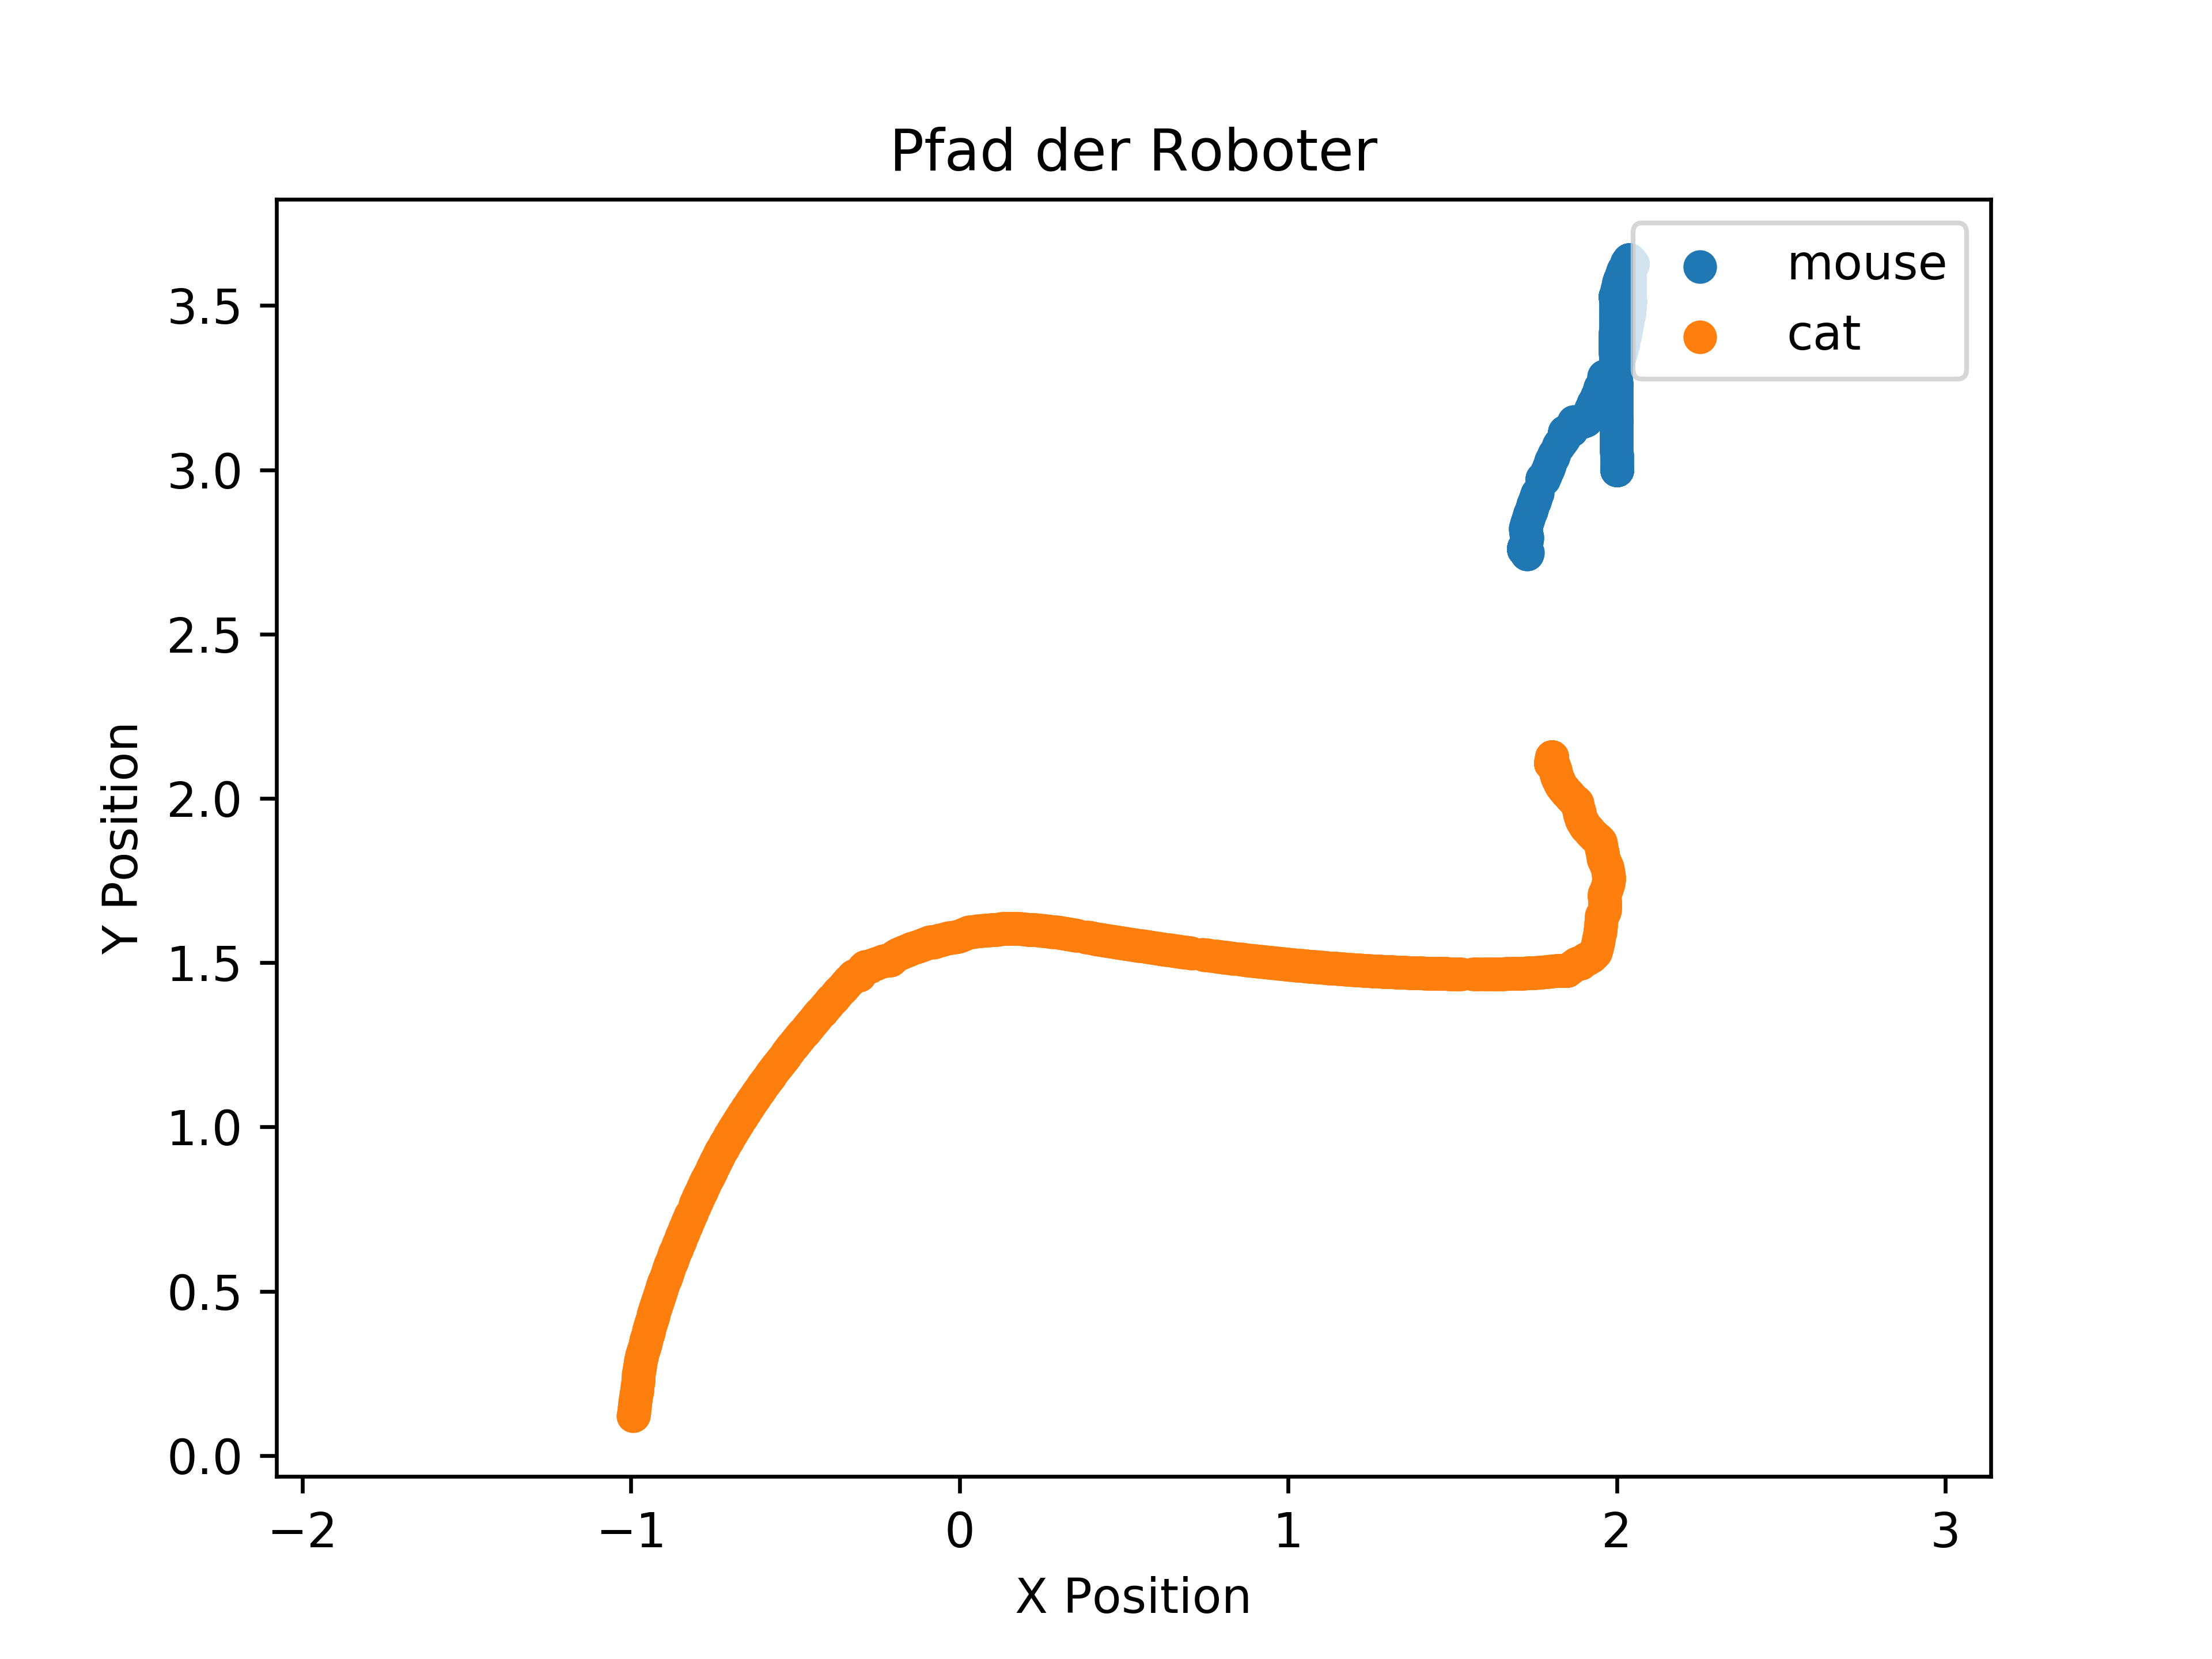
\includegraphics[width=\textwidth]{report_pfad.png}
    \caption{Pfad der Roboter bei Verhaltensfusion}
    \label{fig:pfadFusion}
\end{figure}
\begin{figure}[]
    \centering
    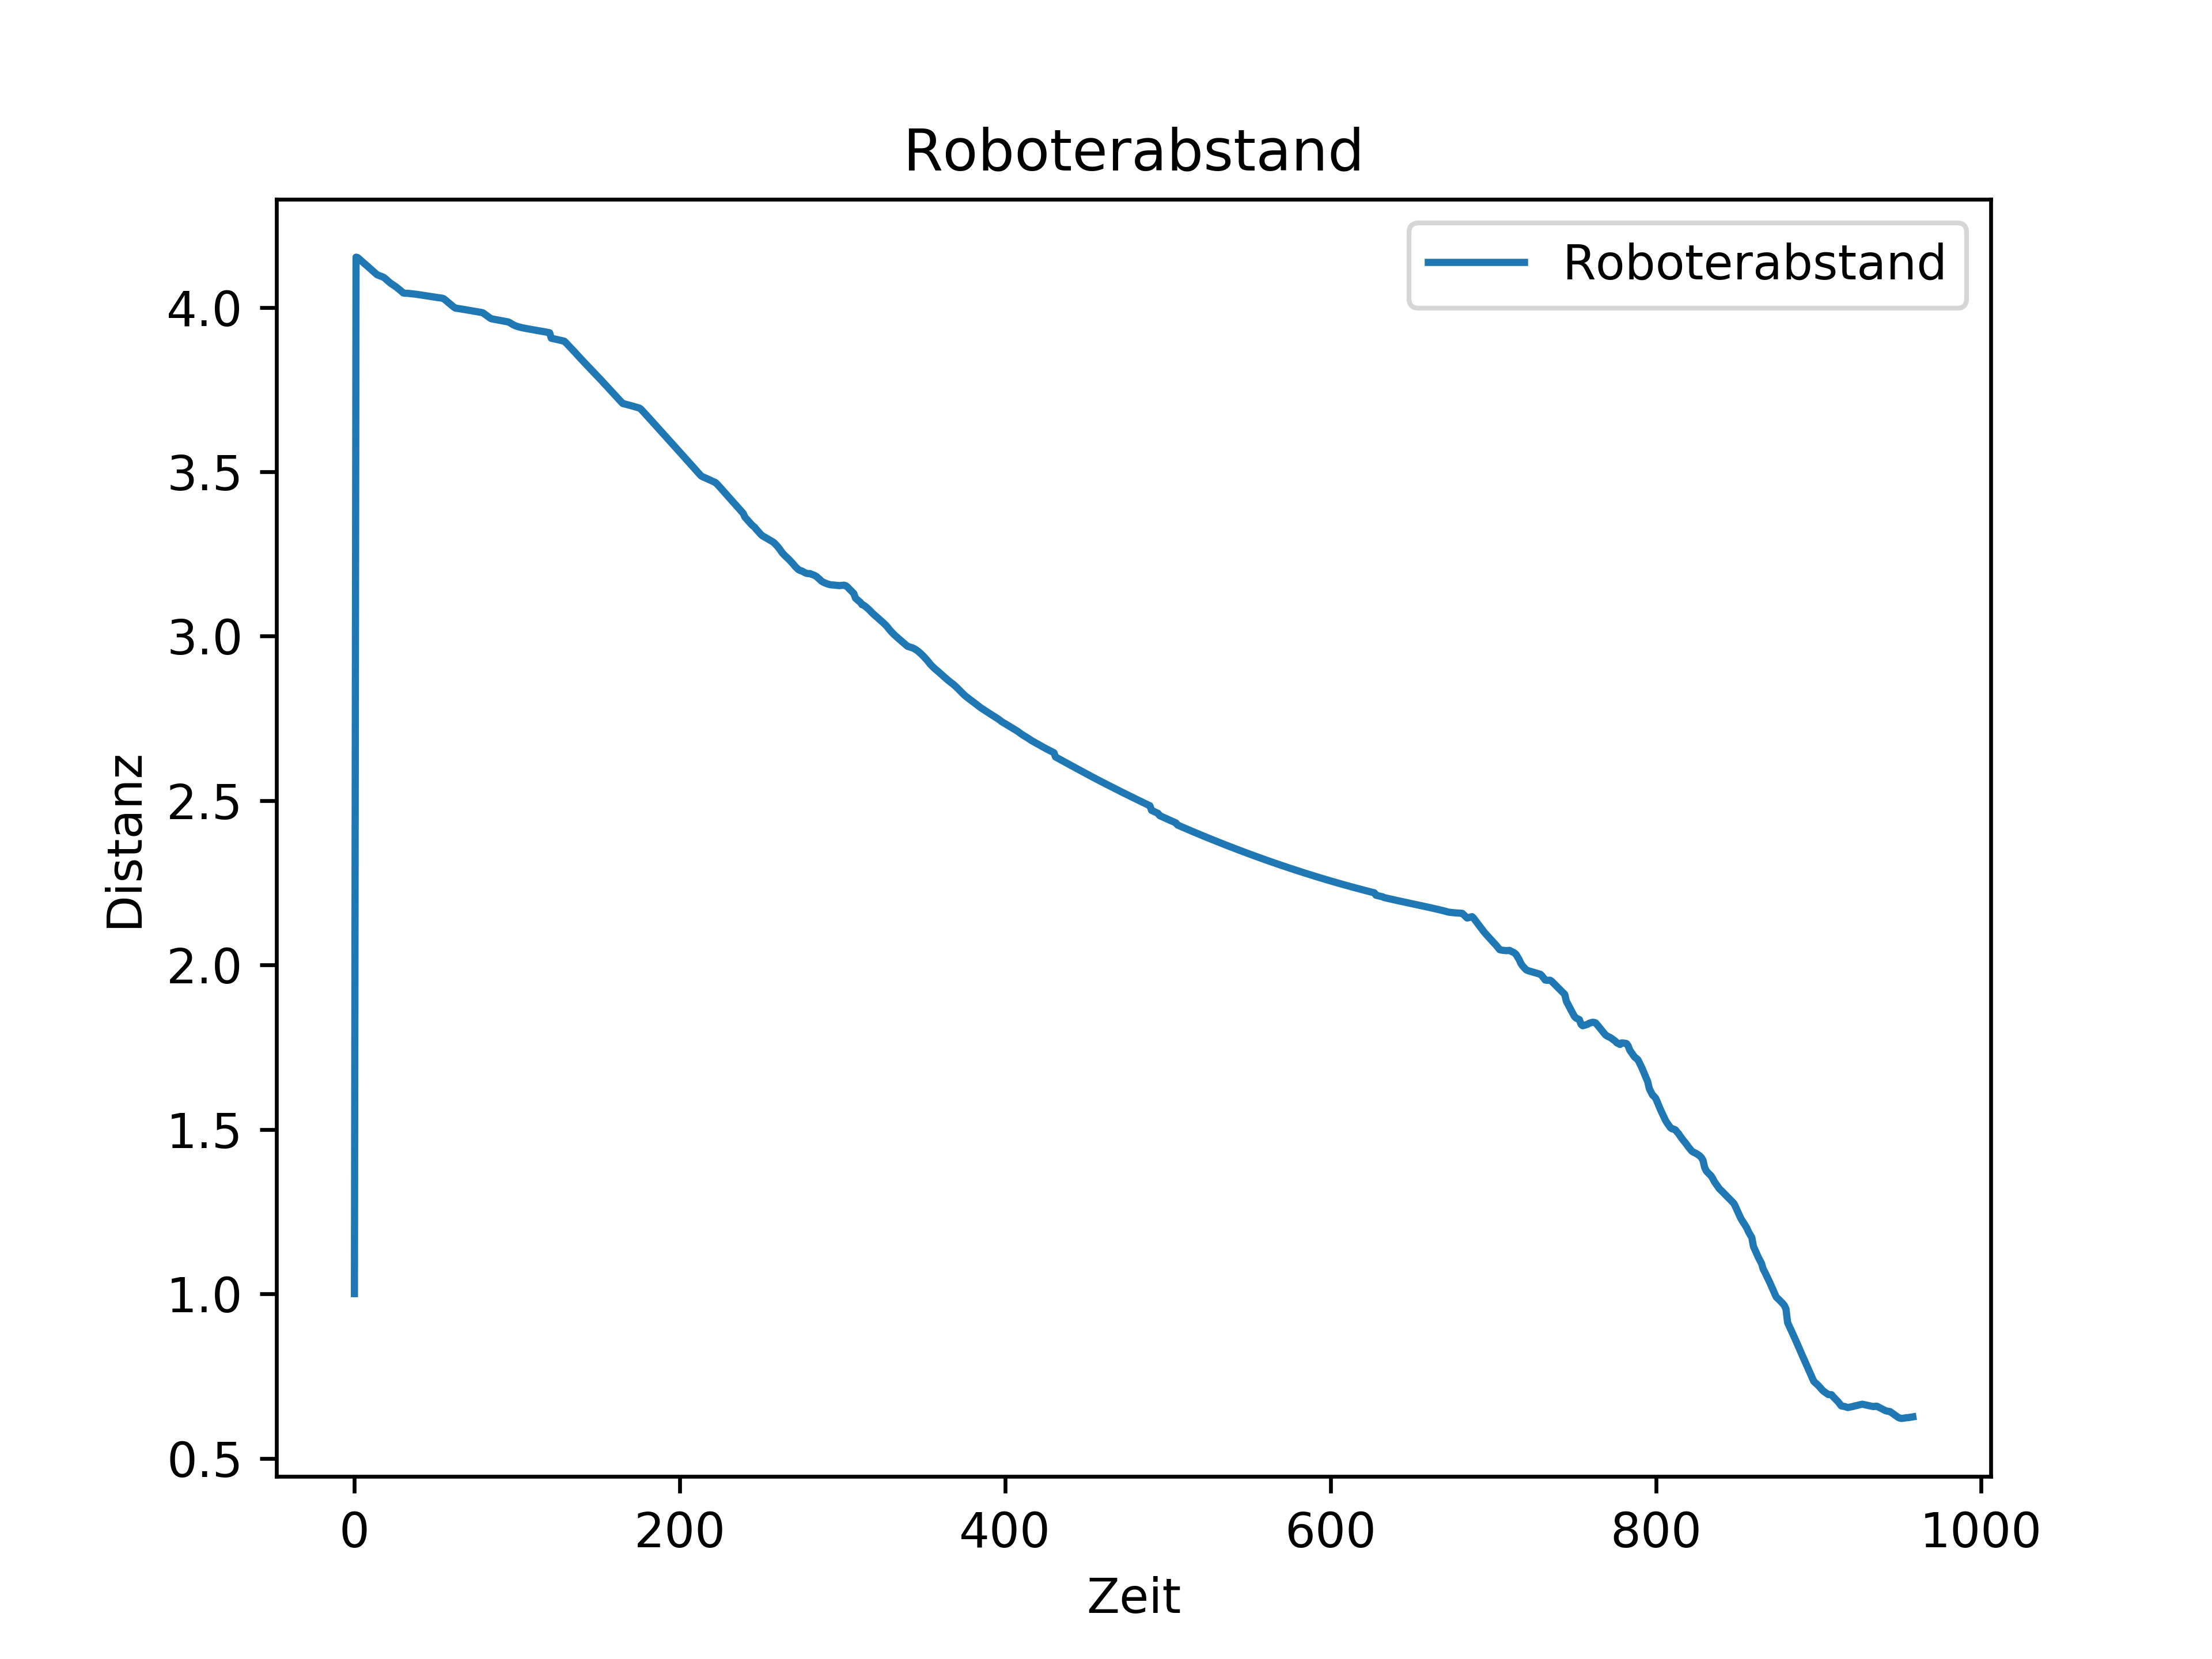
\includegraphics[width=\textwidth]{report_distance.png}
    \caption{Entfernung zwischen den Robotern}
    \label{fig:distanceFusion}
\end{figure}
Der Pfad der Katze in \ref{fig:pfadFusion} verläuft optimal, um die Maus zu erreichen. Bei 0|2 bis ungefähr 1.5|2 begindet sich ein Hinderniss, das umfahren wird, um dann wieder zur Maus aufzuschließen. Dies zeigt sich auch in der linear kleiner werdenden Entfernung zwischen den beiden Robotern. Die Distanz wird nicht auf 0 runter gehen, da in der aktuellen Implementierung die Maus auch als Hindernis erkannt wird und demnach die Kollisionsvermeidung Vorrang erhält, wenn sich die Katze zu sehr der Maus annähert.


\subsection*{Ausblick} \label{chap:ausblick}
Ein sinnvoller Ansatz, der evaluiert werden kann, besteht in der Benutzung von Zusammengesetzten (Compound) Netzwerken. Dabei befindet sich der Roboter in verschiedenen Modi und hat je nach Modi unterschiedliche Verhaltensfusionen. Ein Modus wäre beispielsweise ein direkter Sichtkontakt zur Maus, sodass die Kollisionsvermeidung ausgeschaltet werden kann und die Katze näher an die Maus heranfahren kann. Im Modus Sichtkontakt unterbrochen würde wiederum die Kollisionsvermeidung aktiv werden und gleichzeitig werden Free Space und Zielsuche anders gewichtet.
\\
Ein weiterer Schritt könnte natürlich sein, einen SLAM Algorithmus zu entwickeln, um während der Verfolgung die Umgebung zu scannen und dann nach genug Informationen über den Raum keine Zielsuche mehr durchzuführen sondern eine Wegplanung über bpsw. einen gitterbasierten Dijkstra Ansatz erfolgt.

\end{document}
